\documentclass[%
 reprint,
 nofootinbib,
 amsmath,amssymb,
 aps,
 floatfix,
]{revtex4-2}

% Packages and macros of the report (included by main.tex)

\usepackage[utf8]{inputenc}
\usepackage{graphicx}
\usepackage{dcolumn}
\usepackage{bm}
\usepackage{enumitem}
\usepackage{comment}
\usepackage{siunitx}
\usepackage{booktabs}
\usepackage{placeins}
\usepackage{hyperref}
\hypersetup{colorlinks = true, linkcolor = blue!55!black, citecolor = blue!55!black, urlcolor = blue!55!black}
\usepackage{amsfonts}
\usepackage{nicefrac}
\usepackage{microtype}
\usepackage{amsmath}
\usepackage{mathtools}
\usepackage{multirow}
\usepackage{xcolor}
\usepackage{xspace}

\renewcommand{\thefigure}{\Roman{figure}}

% unit / symbol macros, mirroring the style used in lhc_anomaly_detection/main.tex
\newcommand{\GeV}{\ensuremath{\,\text{Ge\hspace{-.08em}V}}\xspace}
\newcommand{\MeV}{\ensuremath{\,\text{Me\hspace{-.08em}V}}\xspace}
\newcommand{\Araw}{\ensuremath{A_{\mathrm{raw}}}\xspace}
\newcommand{\ACP}{\ensuremath{A_{CP}}\xspace}

% Left-aligned, justified cell of fixed width inside a tabular (replaces p{...} columns, which revtex4-2 breaks with array >= 2.7)
\newcommand{\pcell}[2]{\parbox[t]{#1}{\leftskip=0pt\rightskip=0pt\parfillskip=0pt plus 1fil\relax #2}}

% TODO markers -- remove once every section has real content
\newcommand{\todo}[1]{\textcolor{red}{\textbf{[TODO: #1]}}}

% allow two wide floats on the top of a page (results figures cited together)
\renewcommand{\dbltopfraction}{0.85}
\renewcommand{\dblfloatpagefraction}{0.7}
\setcounter{dbltopnumber}{3}

\usepackage{xspace}\newcommand{\appref}[1]{\unskip~(Appendix~\ref{#1})\xspace}\newcommand{\apprefs}[2]{\unskip~(Appendices~\ref{#1} and~\ref{#2})\xspace}\newcommand{\secorapp}[2]{App.~\ref{#2}}\newcommand{\apponly}[1]{App.~\ref{#1}}\newcommand{\appfig}[2]{\unskip~(Appendix~\ref{#1}, #2)\xspace}\newcommand{\appfigs}[4]{\unskip~(Appendix~\ref{#1}, #2; Appendix~\ref{#3}, #4)\xspace}\newcommand{\apprefsf}[3]{\unskip~(Appendices~\ref{#1} and~\ref{#2}, #3)\xspace}\newcommand{\bnum}[1]{\textbf{\boldmath$#1$}}

\begin{document}
\pagestyle{plain}

\title{Frequentist and Bayesian Analysis of the Matter--Antimatter Asymmetry in $B^{\pm} \to K^{\pm} K^{+} K^{-}$ Decays at LHCb\\[2.0ex]
\small Final project for the \textit{Statistics and Data Analysis} course\\
\small Academic Year 2025--2026}

\author{Marco Belotti}
\author{Giacomo Moretti}
\affiliation{Università degli Studi di Milano-Bicocca}


\begin{abstract}
We measure the raw charge asymmetry $\Araw=[N(B^-)-N(B^+)]/[N(B^-)+N(B^+)]$ of $B^{\pm}\to K^{\pm}K^{+}K^{-}$ decays in the 2011 LHCb Open Data record with an extended unbinned maximum-likelihood fit and with a Bayesian analysis of the same likelihood. On $19{,}731$ candidates we find \bnum{\Araw=-0.0441\pm0.0085\,(\text{stat})\pm0.0072\,(\text{syst})} (Frequentist) and \bnum{-0.0443\pm0.0085\pm0.0070} (Bayesian), \textbf{5.2 standard deviations} from zero. The methods agree in value, uncertainty and coverage, as verified on toy-MC experiments, and the dominant systematic uncertainty is the \emph{particle-identification requirement}. In the Dalitz region of the published analysis we find \bnum{-0.234\pm0.025}, reproducing $-0.239\pm0.020$. A machine-learning selection trained on weak labels leaves $\Araw$ unchanged within its statistical spread. $\Araw$ is not corrected for production and detection asymmetries and is not a measurement of $\ACP$.
\end{abstract}

\maketitle

\section{Introduction}
\label{sec:intro}
The observable of this work is the raw charge asymmetry of the signal yields of $B^{\pm}\to K^{\pm}K^{+}K^{-}$ decays,
\begin{equation}
\Araw=\frac{N(B^-)-N(B^+)}{N(B^-)+N(B^+)} ,
\label{eq:araw}
\end{equation}
which in three-body charmless $B$ decays can be studied globally and locally over the Dalitz plane~\cite{lhcb_cpv_prd2023,lhcb_cpv_paper}. It differs from the $CP$ asymmetry $\ACP$ by the production asymmetry $A_P$ of $B^\pm$ in $pp$ collisions and by the detection asymmetry $A_D$ of the final state~\cite{lhcb_cpv_prd2023},
\begin{equation}
\ACP\approx\Araw-A_P-A_D .
\label{eq:acp}
\end{equation}
Neither correction is applied here, so $\Araw$ is \emph{not} a measurement of $\ACP$; the corrections of the published analysis are discussed in Sec.~\ref{sec:comparison_published}.
We use the LHCb Open Data record for this decay~\cite{opendata_record,opendata_notebook}, a subset of the 2011 data on which the first evidence of an inclusive $CP$ asymmetry was published~\cite{lhcb_cpv_2013}, to ask: \emph{to what extent do Frequentist likelihood fits and Bayesian inference produce consistent, well-controlled estimates of $\Araw$?} The aim is a methodological comparison of the two frameworks on the same data and on the same likelihood, so that any difference comes from the inference and not from the model; the record lacks the control channel needed for $A_P$ and $A_D$\appref{sec:limitations}. Secs.~\ref{sec:data}--\ref{sec:model} describe the data and the common model, Secs.~\ref{sec:frequentist}--\ref{sec:bayesian} the two fits, and Sec.~\ref{sec:validation} the validation of the estimator and of the intervals, Sec.~\ref{sec:ml_body} the machine-learning analysis, Sec.~\ref{sec:dalitz} the Dalitz plane, Sec.~\ref{sec:syst} the systematic study and the result, and Sec.~\ref{sec:comparison} the comparison. The main results are in Table~\ref{tab:summary}.

\begin{table*}[t]
\centering
\begin{tabular}{llcccc}
\toprule
Method & Sample & $\Araw$ & Statistical & Systematic & Section \\
\midrule
Counting (no fit) & fit window, $19{,}731$ & $-0.0432$ & $0.0071$ & -- & \ref{sec:data_exploration} \\
Frequentist fit & fit window, $19{,}731$ & $-0.0441$ & $0.0085$ & $0.0072$ & \ref{sec:frequentist}, \ref{sec:syst} \\
Bayesian fit & fit window, $19{,}731$ & $-0.0443$ & $0.0085$ & $0.0070$ & \ref{sec:bayesian}, \ref{sec:syst} \\
Bayesian fit, $D^0$ veto & $18{,}744$ & $-0.0496$ & $0.0088$ & -- & \apponly{sec:bayes_checks} \\
Bayesian fit, ML selection & score $>0.5$, $15{,}709$ & $-0.0451$ & $0.0087$ & -- & \ref{sec:ml_stability_body} \\
Frequentist fit, ML selection & score $>0.5$, $15{,}709$ & $-0.0447$ & $0.0086$ & -- & \ref{sec:ml_stability_body} \\
Bayesian fit, Dalitz region of Ref.~\cite{lhcb_cpv_2013} & $2146$ & $-0.234$ & $0.025$ & -- & \ref{sec:dalitz} \\
\midrule
Published analysis (same data)~\cite{lhcb_cpv_2013} & different selection and model & $-0.060$ & $0.007$ & -- & -- \\
\bottomrule
\end{tabular}
\caption{Summary of the raw asymmetry $\Araw$ (not corrected for production and detection asymmetries). The Bayesian value is the posterior median and its standard deviation; the systematic uncertainty is given only for the nominal fits (Sec.~\ref{sec:syst}). The published $\Araw$ comes from a different selection and a model with additional background components, so it is not directly comparable with the first rows.}
\label{tab:summary}
\end{table*}


\section{Data}
\label{sec:data}
\emph{In short: the record, the common preselection ($23{,}895$ candidates) and the fit window ($19{,}731$ candidates); the spectrum peaks at $5284\,\MeV$ for both charges and both polarities, and the counting asymmetry is $-0.043\pm0.007$.}
\subsection{Dataset, Preselection and Mass}
\label{sec:data_presel}
The dataset is the CERN Open Data record 4900~\cite{opendata_record}: $B^{\pm}\to h^{\pm}h^{+}h^{-}$ candidates collected by LHCb in 2011 at $\sqrt{s}=7$\,TeV, already through trigger and offline selection, split by magnet polarity ($8{,}556{,}118$ candidates), and a detector-free phase-space simulation of $B^{\pm}\to K^{\pm}K^{+}K^{-}$ ($50{,}000$ decays, no asymmetry) used only to test the local-asymmetry procedure (Sec.~\ref{sec:dalitz}). The same preselection is used in all analyses,
\[
\texttt{H*\_ProbPi} < 0.5 \ \wedge\ \texttt{H*\_ProbK} > 0.5 \ \wedge\ \lnot\texttt{H*\_isMuon},
\]
for each of the three tracks, and retains $23{,}895$ candidates ($0.28\%$). $H1$ is always the kaon of charge opposite to the $B$ and $H2$, $H3$ are the same-sign pair, so the Dalitz variables are the two opposite-sign invariant masses $m^2(H1,H2)$ and $m^2(H1,H3)$.
\label{sec:data_mass}
The three tracks are assigned the charged-kaon mass and their four-momenta are summed to reconstruct $m(KKK)$. The \textbf{nominal fit window}, common to the two analyses, is $[5100,5600]\,\MeV$ and contains $19{,}731$ candidates ($11{,}636$ magnet down, $8095$ magnet up). Below $\sim$5150\,\MeV\ the background rises, which a single exponential cannot describe; the window includes the start of this rise, described by a second exponential in the background model (Secs.~\ref{sec:frequentist}--\ref{sec:bayesian}).
\subsection{Data Exploration}
\label{sec:data_exploration}

Figure~\ref{fig:mass_spectrum} shows the spectrum in the fit window. The peak at $m\approx5284\,\MeV$ over a falling combinatorial background has the same shape for the two charges and the two polarities, which allows a mass and a resolution common to $B^+$ and $B^-$ in the model (Sec.~\ref{sec:model}). The \emph{counting asymmetry} of all candidates, signal and background together, is $A_{\mathrm{count}}=(N^--N^+)/(N^-+N^+)=-0.043\pm0.007$ (binomial uncertainty); the fits of Secs.~\ref{sec:frequentist} and \ref{sec:bayesian} refine it by separating signal and background.

\begin{figure}[t]
\centering
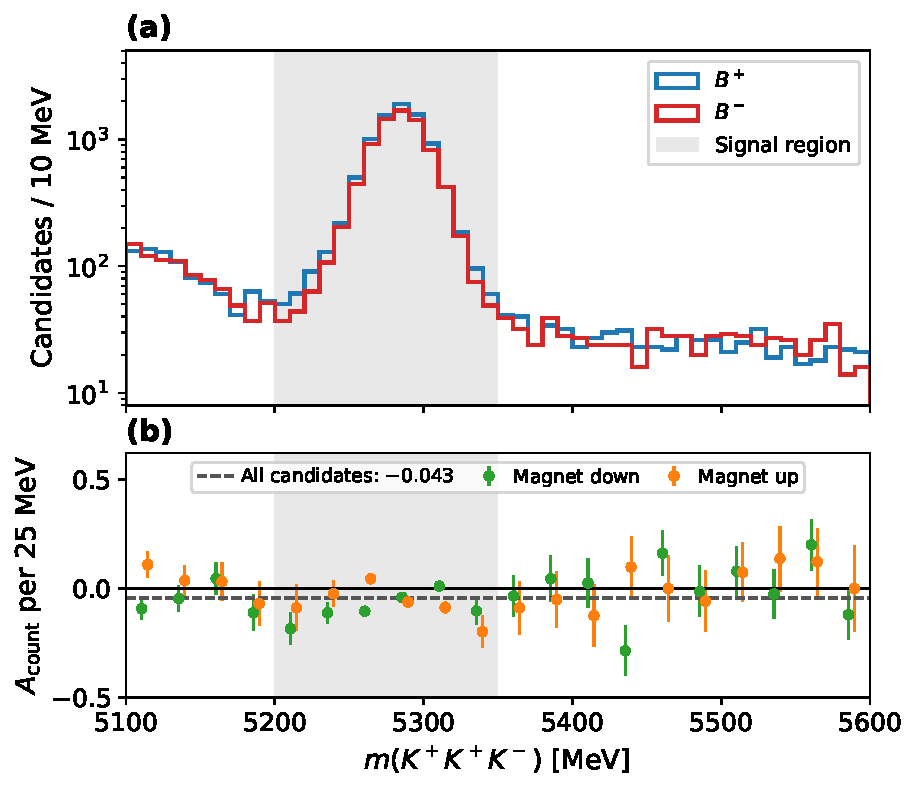
\includegraphics[width=\columnwidth]{figures/mass_spectrum_col.pdf}
\caption{(a) Reconstructed $B\to KKK$ invariant mass in the nominal fit window $[5100,5600]\,\MeV$ for $B^+$ and $B^-$, logarithmic scale; the signal region $[5200,5350]\,\MeV$ is shaded. (b) Counting asymmetry in $25\,\MeV$ bins of the mass for the two magnet polarities, and for all candidates (dashed); the two polarities agree within their uncertainties and the asymmetry is similar in the peak and in the sidebands.}
\label{fig:mass_spectrum}
\end{figure}

\subsection{Additional Results}

\emph{Selection.} The kaon-identification requirement on the three tracks is by far the most selective step of the preselection, and only $42$ candidates of the fit window ($0.2\%$) share a track with another candidate; all are kept.

\section{Mass Model and Likelihood}
\label{sec:model}
\label{sec:bayes_model}
\emph{In short: one extended likelihood shared by the two analyses: a Gaussian signal with common mean and width, a double-exponential background for each charge and $A$ as a parameter.}
The mass spectrum of each charge sample is described by a signal-plus-background mixture on the nominal fit window $[5100,5600]\,\MeV$ (Sec.~\ref{sec:data_mass}),
\begin{equation}
f^{\pm}(m)=N_s^{\pm}\,S(m;\mu,\sigma)+N_b^{\pm}\,B^{\pm}(m),
\label{eq:mixture}
\end{equation}
where $S$ is a Gaussian truncated to the window, with mean $\mu$ and width $\sigma$ shared by the two charges, and the background is a double exponential with a shape of its own for each charge,
\[
B^{\pm}(m)=f_{\pm}\,E(m;\lambda_{1}^{\pm})+(1-f_{\pm})\,E(m;\lambda_{2}^{\pm}),
\]
with $E(m;\lambda)\propto e^{-\lambda m}$ a truncated exponential normalized on the window. The steep component ($\lambda_1$) describes the rise of the background towards the lower edge of the window, the slow one ($\lambda_2$) the combinatorial background under and above the peak. The ordering $\lambda_1>\lambda_2$ removes the label-switching symmetry of the mixture (exchanging the two exponentials would give two identical modes). Signal and background yields are split between the charges as
\[
N_s^{\pm}=\tfrac{N_s}{2}(1\mp A),\qquad N_b^{\pm}=\tfrac{N_b}{2}(1\mp A_b),
\]
so that $A=(N_s^--N_s^+)/(N_s^-+N_s^+)$, the raw asymmetry \Araw of Eq.~\eqref{eq:araw}, is itself a parameter of the fit, the \emph{parameter of interest} (POI, all the others being nuisance parameters), and the background asymmetry $A_b$ is free. The parameter vector has twelve components, $\theta=(N_s,N_b,A,A_b,\mu,\sigma,\lambda_1^{\pm},\lambda_2^{\pm},f_{\pm})$.
Given the data $D=\{(m_i,q_i)\}_{i=1}^{N}$ (mass and charge of each candidate), the extended unbinned likelihood of the two charge samples is
\begin{multline}
\mathcal{L}(D\mid\theta)\propto e^{-(N_s+N_b)}
\prod_{i:\,q_i=+1}\Big[N_s^{+}S(m_i)+N_b^{+}B^{+}(m_i)\Big] \\
\times\prod_{i:\,q_i=-1}\Big[N_s^{-}S(m_i)+N_b^{-}B^{-}(m_i)\Big],
\label{eq:likelihood}
\end{multline}
where $S(m_i)\equiv S(m_i;\mu,\sigma)$. The likelihood is \emph{extended} (the yields are parameters, hence the Poisson term); it is the common ground of the two mass analyses: Sec.~\ref{sec:frequentist} maximizes it and Sec.~\ref{sec:bayesian} multiplies it by a prior. Since both use this model unchanged, any difference between their results can only come from \emph{the inference}.
\subsection{Additional Results}
\emph{Minimal model.} A six-parameter model on a narrower window gives $\Araw=-0.0497$ ($68\%$ Confidence Interval $[-0.058,-0.041]$), compatible with the nominal result within its uncertainty.

\section{Frequentist Analysis}
\label{sec:frequentist}
\emph{In short: the likelihood maximized for the two charges together gives $N_s=15{,}328\pm133$ and $\hat A=-0.0441$ with Minos intervals; $A=0$ is rejected at $5.2\sigma$ and the interval has nominal coverage in $1000$ bootstrap replicas.}
The Frequentist analysis estimates \Araw by maximizing the extended unbinned likelihood of Eq.~\eqref{eq:likelihood} with \texttt{iminuit}~\cite{iminuit}; the uncertainty and the test of $A=0$ come from the profile likelihood, the other parameters being nuisance parameters (Secs.~\ref{sec:freq_model}--\ref{sec:freq_ci}).
\subsection{Mass Model and Fit Strategy}
\label{sec:freq_model}
\label{sec:freq_simfit}
The common mass model of Sec.~\ref{sec:model} (Eq.~\eqref{eq:mixture}) was fitted on $[5100,5600]\,\MeV$: a Gaussian signal with mean $\mu$ and width $\sigma$ shared by the two charges and a double-exponential background with shape and yield of its own for each charge, twelve parameters as in the Bayesian fit, through \texttt{iminuit.cost.ExtendedUnbinnedNLL}; the minimization started from an unbinned fit of the sidebands (the window without $[5200,5350]\,\MeV$). The asymmetry was estimated in two ways: in the \emph{simultaneous} fit the two charges share $N_s^\pm=N_s(1\mp A)/2$ and $A$ is a parameter of the likelihood; in the \emph{separate} fits each charge was fitted alone (seven free parameters each) and $\Araw=(N_s^--N_s^+)/(N_s^-+N_s^+)$ was computed from the two yields. They give $-0.0441\pm0.0085$ and $-0.0442\pm0.0087$: sharing $\mu$ and $\sigma$ between a particle and its antiparticle is adequate, and the simultaneous fit, which gives the profile-likelihood interval directly, is the \textbf{nominal} one. It gives $N_s=15{,}328\pm133$ and $N_b=4403\pm82$, against the Bayesian posterior medians $15{,}328\pm133$ and $4404\pm82$ (Sec.~\ref{sec:bayes_posterior}). The nominal fit has $\chi^2/\mathrm{ndof}=160/88$ ($p=4.8\cdot 10^{-6}$) in $2\times50$ bins of $10\,\MeV$; a single exponential is rejected ($294/92$, $p=5.7\cdot 10^{-23}$) because the background rises towards the lower edge of the window (Sec.~\ref{sec:data_mass}). The fit of the two charges is shown in Fig.~\ref{fig:freq_jointfit}.

\begin{figure*}[t]
\centering
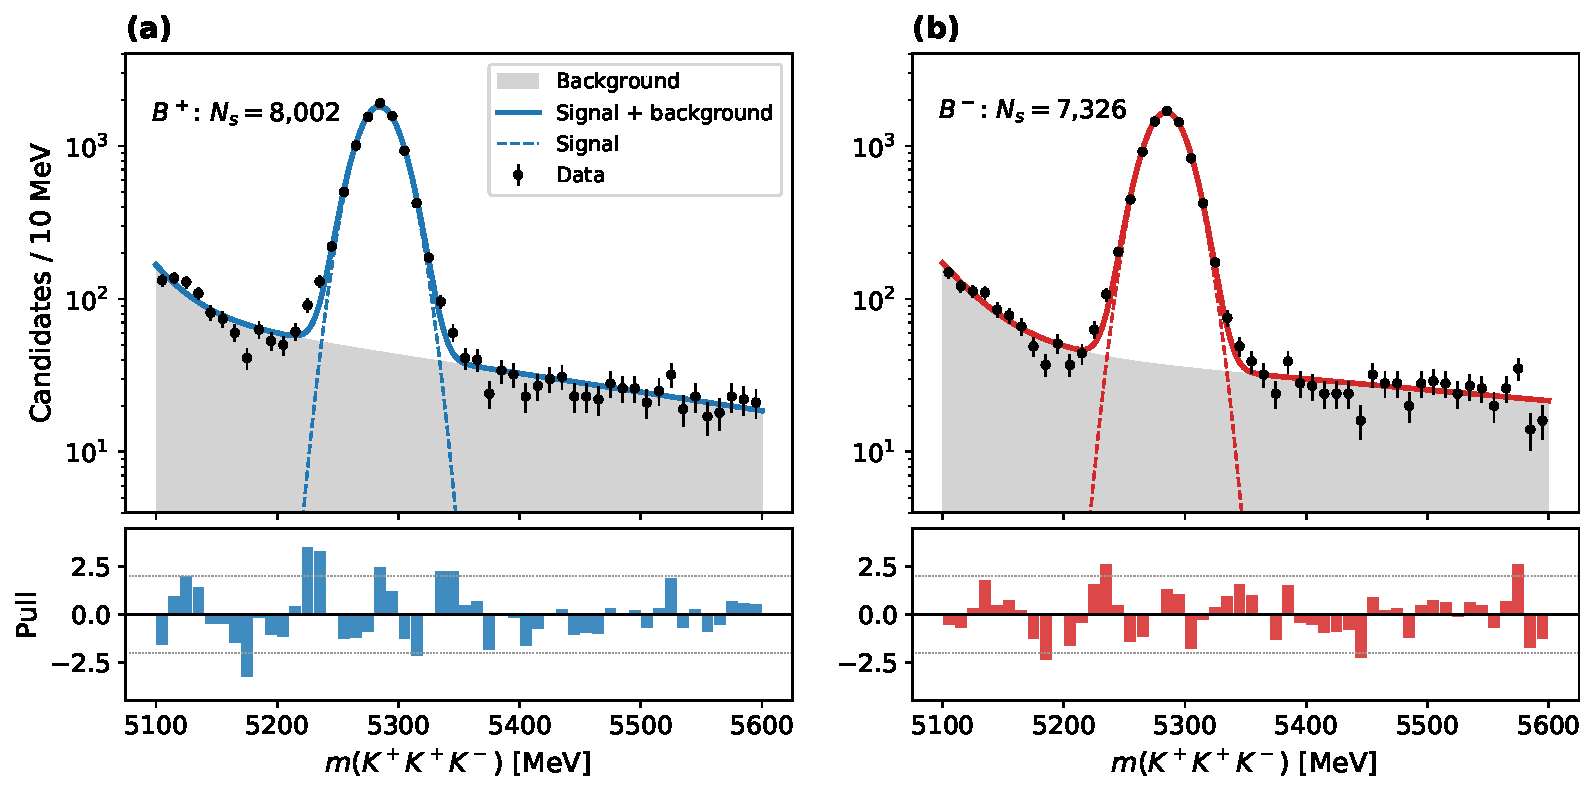
\includegraphics[width=0.95\textwidth]{figures/freq_jointfit.pdf}
\caption{Simultaneous fit of (a) $B^+$ and (b) $B^-$ in $10\,\MeV$ bins, logarithmic scale: data, signal (dashed), double-exponential background (grey) and their sum; below, the pulls $(n_i-\mu_i)/\sqrt{\mu_i}$ of the fit, with the $\pm2$ lines. The fitted signal yields are $8002$ and $7326$.}
\label{fig:freq_jointfit}
\end{figure*}

\subsection{Profile Likelihood and Confidence Interval}
\label{sec:freq_ci}
The maximum-likelihood estimate is \bnum{\hat A=-0.0441} (Hesse uncertainty $0.0085$), with \texttt{MINOS}~\cite{minuit} intervals $68\%$ CI $[-0.0526,-0.0356]$ and $95\%$ CI $[-0.0607,-0.0275]$; the uncertainties are statistical only (the systematic one is in Sec.~\ref{sec:syst}). The \emph{profile likelihood ratio} $q(A)=-2\log[L(A,\hat{\hat\theta})/L(\hat A,\hat\theta)]$, with the other eleven parameters re-minimized at each $A$ (\texttt{mnprofile}), is shown in Fig.~\ref{fig:freq_profile}; by Wilks' theorem~\cite{wilks} it follows a $\chi^2$ distribution with one degree of freedom at the true value of $A$, so the intervals are the sets $q\leq1$ and $q\leq3.84$. For the null hypothesis, $q(0)\simeq27$, $p=2.05\times10^{-7}$, \bnum{5.20\sigma}: no asymmetry is rejected, the counterpart of the Savage-Dickey test of Sec.~\ref{sec:bayes_factor} ($A=0$ at $5.2$ posterior standard deviations); the $p$-value is not the probability of $H_0$ and the Bayes factor depends on the prior width, but the conclusion is the same. The result agrees with the Bayesian one (Sec.~\ref{sec:bayes_posterior}: $-0.0443$, $68\%$ CI $[-0.0528,-0.0358]$), as expected with flat priors and $\sim2\times10^4$ events.

\begin{figure}[h]
\centering
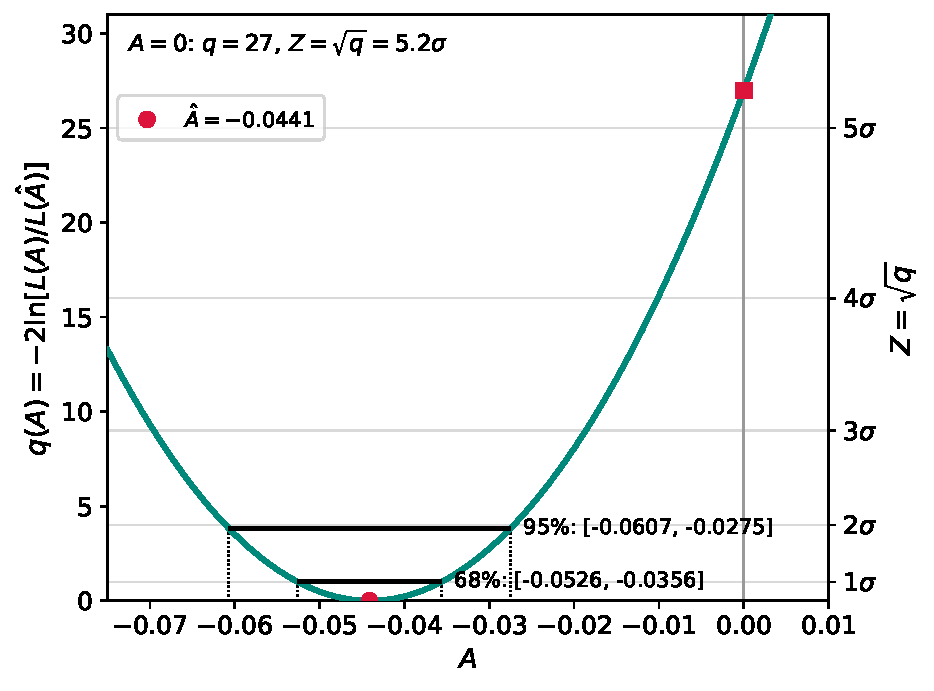
\includegraphics[width=\columnwidth]{figures/freq_profile.pdf}
\caption{Profile likelihood ratio $q(A)$ of the simultaneous fit, with the other eleven parameters re-minimized at each $A$ (right axis: $Z=\sqrt q$). The horizontal segments are the $68\%$ and $95\%$ Minos intervals ($q\leq1$, $q\leq3.84$); at $A=0$, $q\simeq27$, i.e. $5.2\sigma$.}
\label{fig:freq_profile}
\end{figure}

\subsection{Coverage of the Wilks Intervals}
\label{sec:freq_coverage}
Wilks' theorem is asymptotic, so the coverage was checked on the data with $1000$ bootstrap replicas of the $19{,}731$ candidates, refitting the nominal model on each (non-converged fits discarded); with $A_{\mathrm{true}}=-0.0441$, the $68\%$ interval of a replica contains it if and only if $q(A_{\mathrm{true}})\leq1$. The fraction is \bnum{68.4\pm1.5\%} against $68.3\%$ nominal (Fig.~\ref{fig:freq_toys}). It agrees with the toy-MC check of the Bayesian interval ($65.0\pm3.3\%$, $200$ experiments); the two checks are not equivalent, since the Bayesian pseudo-datasets come from the fitted model (a closure test) while the replicas are resampled from the data and carry the features that the model does not describe, such as the signal tails.

\begin{figure}[h]
\centering
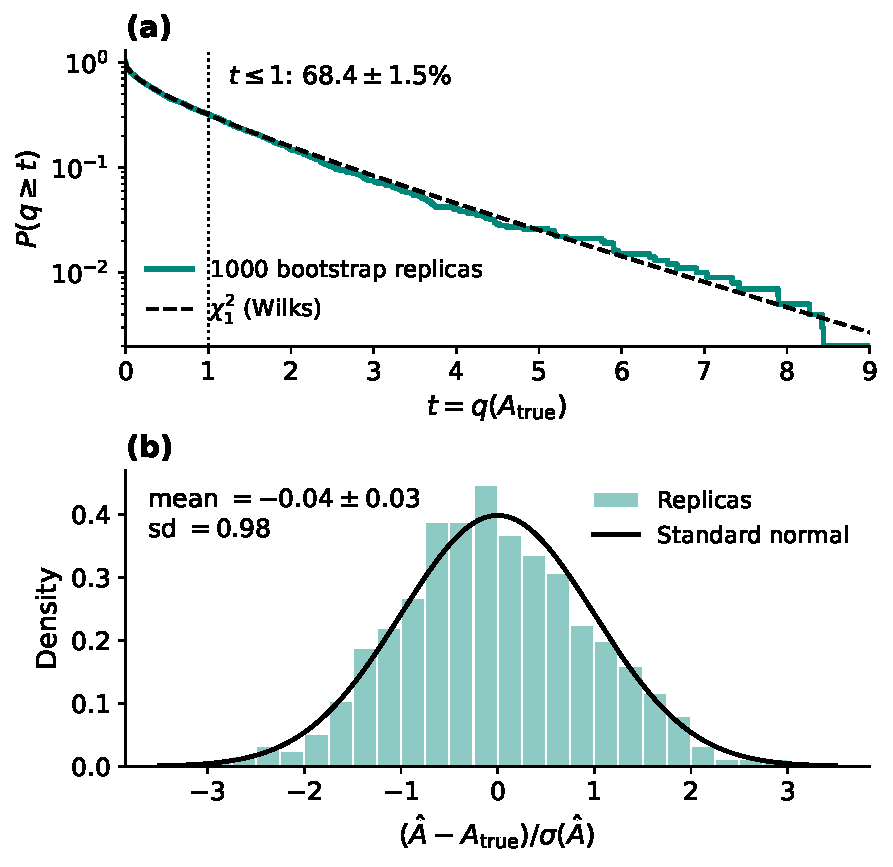
\includegraphics[width=\columnwidth]{figures/short_coverage.pdf}
\caption{Coverage check with $1000$ bootstrap replicas of the data. (a) Survival function of $t=q(A_{\mathrm{true}})$ against the $\chi^2_1$ distribution expected from Wilks' theorem; the dotted line is the $68.3\%$ limit ($t=1$). (b) Pulls $(\hat A-A_{\mathrm{true}})/\sigma(\hat A)$ of the replicas against a standard normal.}
\label{fig:freq_toys}
\end{figure}

\subsection{Additional Results}
\emph{Neyman belt construction and momentum.} Inverting the test of $A_{\mathrm{true}}$ with toy-MC experiments gives the same interval as the likelihood ratio, and $\Araw$ does not depend on the momentum of the $B$.
\emph{Uncertainties of the twelve parameters.} The standard deviations from the Hesse matrix, the bootstrap of the data and the posterior agree for $A$, $A_b$, $\mu$ and $\sigma$; the bootstrap differs for the two yields, because it keeps the total number of candidates fixed, and for the weakly constrained steep slope $\lambda_1^+$.

\section{Bayesian Analysis}
\label{sec:bayesian}
\emph{In short: the same likelihood with uniform priors, sampled with MCMC: $\Araw=-0.0443$ ($68\%$ interval $[-0.0528,-0.0358]$) with converged chains; the Bayes factor of $A=0$, $BF_{10}\approx9\times10^3$, depends on the prior width.}
The Bayesian analysis takes the likelihood of Sec.~\ref{sec:model} as it is and adds only a prior and a sampler; it changes the question asked of the data, not the model.
\subsection{Priors and Posterior}
\label{sec:bayes_prior}
Bayes' theorem combines the likelihood of Eq.~\eqref{eq:likelihood} (Sec.~\ref{sec:model}) with a prior $\pi(\theta)$ into the posterior
\begin{equation}
p(\theta\mid D)=\frac{\mathcal{L}(D\mid\theta)\,\pi(\theta)}{p(D)},
\label{eq:bayes}
\end{equation}
The priors are uniform, with independent ranges except for the ordering of the background slopes: $N_s,N_b\in(0,5N)$ with $N=19{,}731$, $A,A_b\in(-1,1)$, $\mu\in(5260,5310)\,\MeV$, $\sigma\in(3,40)\,\MeV$, $\lambda_1^{\pm}\in(10^{-5},0.1)\,\MeV^{-1}$, $\lambda_2^{\pm}\in(10^{-5},\lambda_1^{\pm})$, $f_{\pm}\in(0,1)$. The prior density is therefore a constant on the allowed region $\Theta$,
\begin{equation}
\pi(\theta)\propto\mathbf{1}\left[\theta\in\Theta\right],
\label{eq:prior}
\end{equation}
and inside it the posterior is proportional to the likelihood. A flat prior is not invariant under reparametrization, but with $\sim$$2\times10^4$ events the posterior is dominated by the likelihood, as a prior-sensitivity check confirms for $A$. The evidence $p(D)$ is a constant: the MCMC samples $\mathcal{L}\,\pi$ without it, and the Savage-Dickey ratio of Sec.~\ref{sec:bayes_factor} avoids it as well; the marginal posterior of $A$ is the histogram of the $A$ component of the chain.
\subsection{MCMC Sampling and Convergence Diagnostics}
\label{sec:bayes_mcmc}
The posterior was sampled with the affine-invariant ensemble sampler of Goodman and Weare~\cite{goodman_weare} as implemented in \texttt{emcee}~\cite{emcee}: 32 walkers started around the maximum of the posterior, $25{,}000$ steps with the first $1/6$ discarded as burn-in ($6.7\times10^5$ samples, acceptance $0.38$). The integrated autocorrelation time is $\tau\in[147,183]$ steps, so the chain is $N/\tau\geq113$ autocorrelation times long for every parameter, above the threshold of $50$~\cite{emcee} ($\gtrsim3600$ effectively independent samples). Two runs started uniformly over the whole prior box converge to the same single mode. The profile likelihood is tabulated so that the result can be combined with others.
\subsection{Posterior Results and Credible Intervals}
\label{sec:bayes_posterior}

The nominal model with the posterior medians coincides with the fit of Fig.~\ref{fig:freq_jointfit}, which it follows over two orders of magnitude. The marginal posterior on the raw asymmetry gives (median and equal-tailed credible intervals, CI)
\begin{gather*}
\Araw = -0.0443, \\
68\%~\text{CI}~[-0.0528,-0.0358], \\ 95\%~\text{CI}~[-0.0608,-0.0276].
\end{gather*}
The posterior is very close to Gaussian (standard deviation $0.0085$), so equal-tailed and highest-posterior-density intervals coincide; with uniform priors its mode, $-0.0441$, is the maximum-likelihood estimate and the result can be compared directly with the Frequentist fit (Sec.~\ref{sec:frequentist}). The other physics parameters (Fig.~\ref{fig:bayes_corner}) are $N_s=15{,}328\pm133$, $N_b=4404\pm82$, $A_b=-0.040\pm0.018$, $\mu=5284.39\pm0.16\,\MeV$ and $\sigma=18.00\pm0.14\,\MeV$. $A$ is almost uncorrelated with them, which is why profiling (Frequentist) and marginalizing (Bayesian) the nuisance parameters give the same result; the largest correlation, $-0.17$, is with $A_b$: conditioning on $A_b=0$ moves $A$ to $-0.0475$, as the fit with a charge-symmetric background does ($-0.0471$, Sec.~\ref{sec:syst}).

\begin{figure*}[t]
\centering
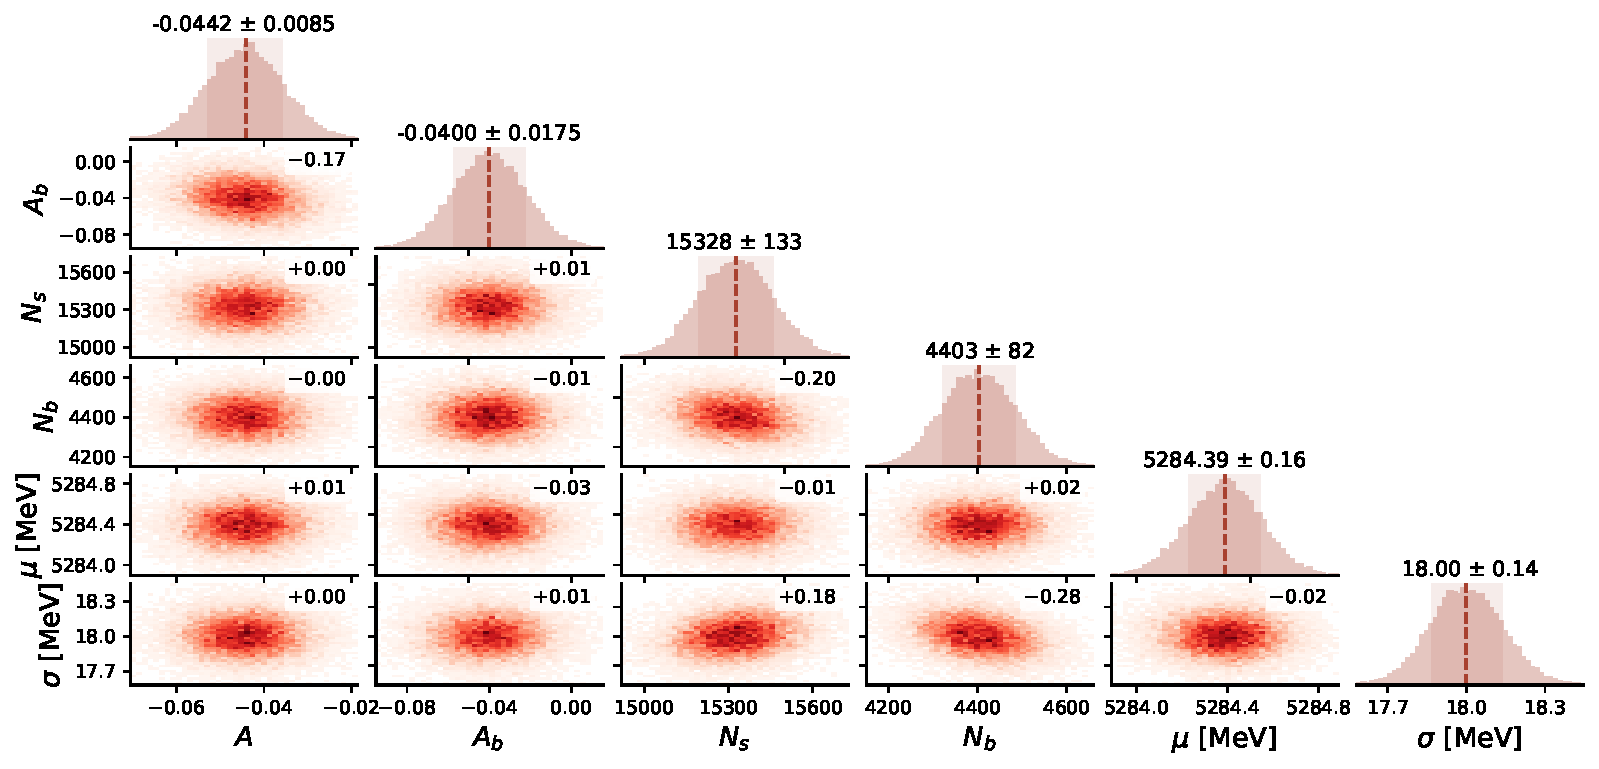
\includegraphics[width=0.78\textwidth]{figures/short_corner.pdf}
\caption{Marginal posteriors and correlations of the six physics parameters of the nominal fit (the six background-shape parameters are marginalized). Diagonal: posterior with its median (line) and $68\%$ interval (band), quoted above as median $\pm$ half-width; below the diagonal: two-dimensional posteriors with the correlation coefficient.}
\label{fig:bayes_corner}
\end{figure*}

\subsection{Bayes Factors}
\label{sec:bayes_factor}
The Bayes factor compares two hypotheses through their evidences, $BF_{10}=P(D\mid H_1)/P(D\mid H_0)$, and requires proper priors. For the nested hypothesis $H_0$: $A=0$ against $H_1$: $A$ free, with shared priors on the other parameters, it reduces to the Savage-Dickey ratio~\cite{dickey1971},
\[
BF_{01} = \frac{p(A=0\mid D)}{\pi(A=0)}, \qquad \pi(A=0)=\tfrac12 .
\]
$A=0$ lies $5.2$ posterior standard deviations from the median, where the chain has essentially no samples, so $p(A=0\mid D)$ was taken from the Gaussian approximation of the marginal posterior: \bnum{BF_{01}\approx1.1\times10^{-4}} ($BF_{10}\approx9\times10^{3}$; Fig.~\ref{fig:bayes_sd}a), \textbf{decisive evidence} against $A=0$ on Jeffreys' scale~\cite{jeffreys}. The value scales with the prior width (Ockham factor): with $A\in(-0.3,0.3)$, $BF_{01}$ drops by a factor $3.3$ and the conclusion is unchanged.

\begin{figure*}[!t]
\centering
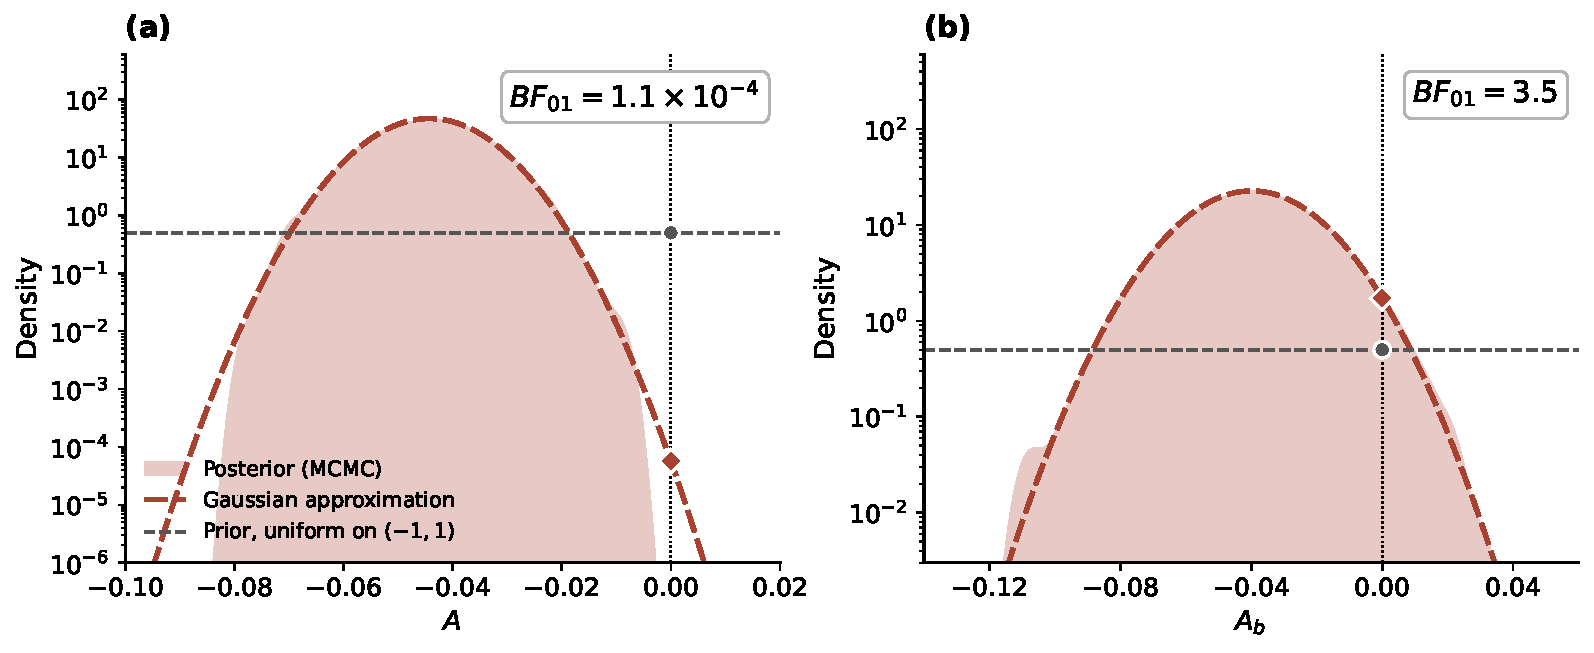
\includegraphics[width=0.78\textwidth]{figures/short_savage_dickey.pdf}
\caption{Savage-Dickey ratio for (a) $A$ and (b) $A_b$: marginal posterior (histogram of the chain and Gaussian approximation) and prior density, logarithmic scale. The Bayes factor $BF_{01}$ is the ratio of the two densities at zero (dots). For $A$ the posterior density at zero is $10^{-4}$ times the prior one; for $A_b$, $2.3$ standard deviations from zero, it is higher than the prior density, and the data favor $A_b=0$.}
\label{fig:bayes_sd}
\end{figure*}

The same test on the background asymmetry shows the Ockham factor at work: $A_b=-0.040\pm0.018$ is $2.3$ standard deviations from zero, yet $BF_{01}(A_b=0)\approx3.5$ (Fig.~\ref{fig:bayes_sd}b), because the likelihood gain does not compensate for spreading the prior; unlike for $A$, the preference changes sign with the prior width. Of the Bayesian results \emph{only the Bayes factor} depends on the prior; the interval of $A$ does not (Sec.~\ref{sec:bayes_posterior}). %A negative $A_b$ is plausible given the misidentified $B^\pm\to K^\pm\pi^+\pi^-$ and $\pi^\pm K^+K^-$ decays;
$A_b$ is kept free in the nominal model and fixing it to zero is one of the systematic variants (Sec.~\ref{sec:syst}).
\subsection{Additional Results}
\emph{Intervals.} Equal-tailed and highest-posterior-density $68\%$ intervals coincide for $A$ and $A_b$ and differ for the skewed parameters; the profile likelihood is tabulated for combination with other results.
\emph{Priors.} No change of the prior on the nuisance parameters or of its parametrization moves $A$ by more than $0.0002$, and the evidence by direct integration agrees in order of magnitude with the Savage-Dickey ratio.
\emph{Model adequacy.} The model does not reach $\chi^2/\mathrm{ndof}\approx1$ ($164.1/88$), because the signal tails are heavier than a Gaussian, but $\Araw$ changes by $-0.0002$ with a Crystal Ball signal; the posterior predictive check reproduces the asymmetry in slices of the mass ($p_B=0.67$, the posterior predictive $p$-value, i.e.\ the fraction of replicas whose discrepancy exceeds the observed one) and puts the difference of the $\chi^2$ of the two charges at the edge of the replicas ($p_B=0.08$).
\emph{Robustness and coverage.} $\Araw$ agrees between the magnet polarities ($0.7\sigma$); $200$ toy-MC experiments give coverage $0.65\pm0.03$ ($68\%$) and $0.93\pm0.02$ ($95\%$) with pulls of width $1.04$.

\section{Validation of the Estimator and of the Intervals}
\label{sec:validation}
\label{sec:validation_estimator}
\emph{In short: toy-MC experiments show an unbiased estimator at the minimum variance bound, intervals with nominal coverage and a test of $A=0$ with the nominal size.}
Toy-MC experiments generated from the fitted model of Sec.~\ref{sec:model} (Poisson yields, masses drawn from the model by the transformation method; $1000$ at the fitted value $A_{\mathrm{true}}=-0.0441$ and $300$ at each of $-0.1$, $-0.02$, $0$ and $+0.05$, each fitted with the nominal procedure, $1$--$3\%$ of the fits not valid and excluded) verify the estimator and the profile-likelihood ratio. Over the five values the bias of $\hat A$ is at most $0.0008$ ($1.6$ standard errors; $-0.0005$, $-0.0001$, $-0.0008$, $+0.0002$, $-0.0004$ for the five values; Fig.~\ref{fig:validation_injection}a), its spread equals the mean Hesse uncertainty within $6\%$ and the pulls have width $0.94$--$1.05$ (Fig.~\ref{fig:validation_injection}b): the estimator is \textbf{unbiased} and reaches the \textbf{minimum variance bound}.
At the fitted value the coverage of $t(A_{\mathrm{true}})\leq1$ is $0.696\pm0.015$ ($68.3\%$ level) and $0.954\pm0.007$ ($95.4\%$ level); the $68\%$ coverage over the five values is $0.71$, $0.70$, $0.69$, $0.69$ and $0.61$. %, the last, at $+0.05$ ($0.614\pm0.028$), $2.5$ standard deviations low, not unexpected among five values.
Inverting the Neyman construction, with $300$ toy-MC experiments at each of $11$ values of $A_{\mathrm{true}}$ between $-0.1$ and $0$, at the observed $\hat A$ gives the $68\%$ interval $[-0.0528,-0.0351]$, against the Minos interval $[-0.0526,-0.0356]$. The test of $A=0$ has the nominal size, $0.051\pm0.013$ at $A_{\mathrm{true}}=0$ against $0.05$, and $q(0)$ is compatible with $\chi^2_1$; Figure~\ref{fig:validation_injection} shows (a) the bias, (b) the spread and the pull width and (c) the size and the power of the test as a function of the injected asymmetry.

\begin{figure*}[!t]
\centering
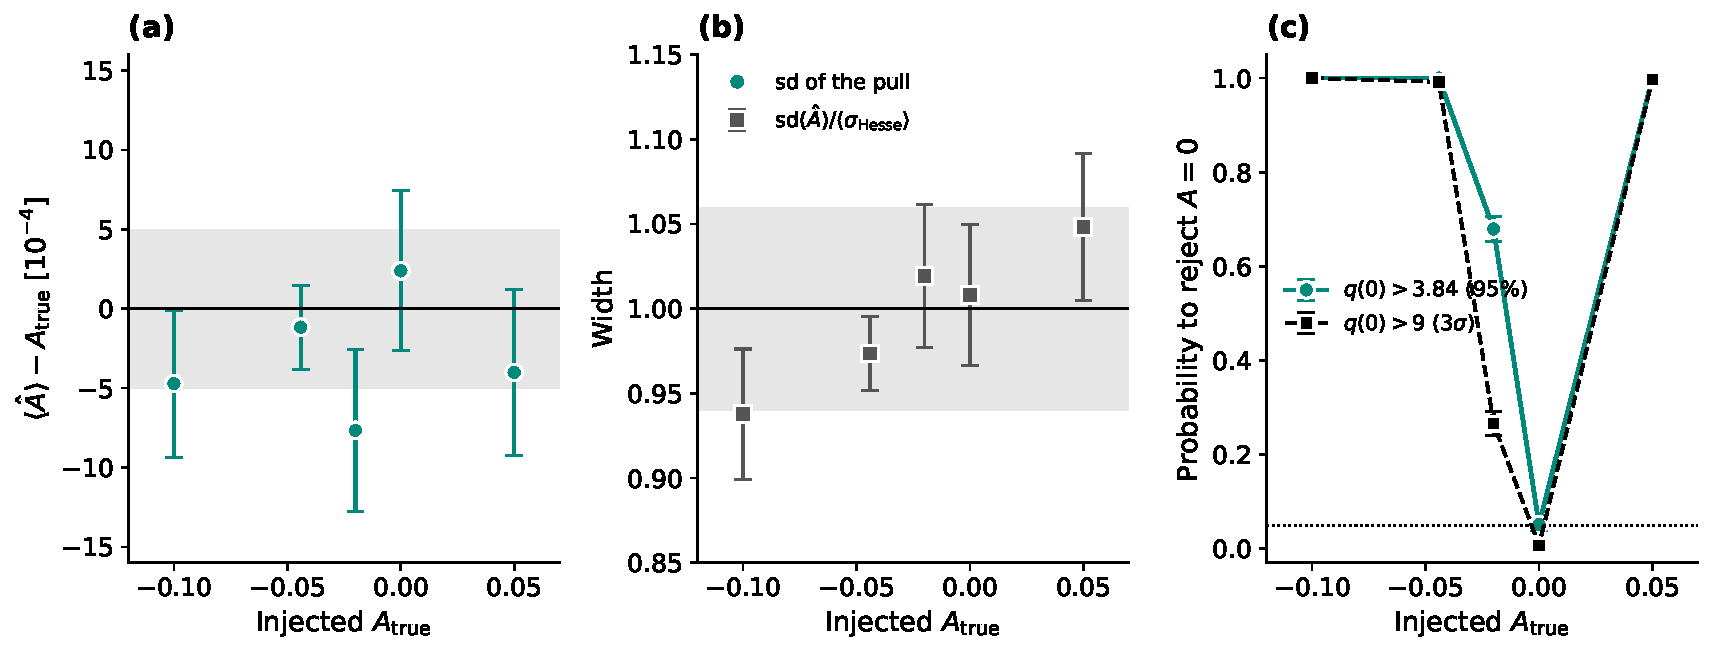
\includegraphics[width=0.95\textwidth]{figures/short_injection_power.pdf}
\caption{Toy-MC experiments at five injected asymmetries. (a) Bias of $\hat A$, with its standard error. (b) Spread of the estimates divided by the mean Hesse uncertainty, and width of the pulls. (c) Probability to reject $A=0$ in the test with $q(0)>3.84$ (size $5\%$) and $q(0)>9$ ($3\sigma$), as a function of the injected value: size at $A_{\mathrm{true}}=0$, power elsewhere.}
\label{fig:validation_injection}
\end{figure*}

%Under $A_{\mathrm{true}}=0$ the test $q(0)>3.84$ rejects in $0.051\pm0.013$ of the experiments, the \textbf{nominal size}, with $q(0)$ compatible with $\chi^2_1$ (Kolmogorov-Smirnov $p=0.79$); its power is $1.00$ at the fitted value and $0.68$ ($0.27$ at $3\sigma$) at $A_{\mathrm{true}}=-0.02$, so with $19{,}731$ candidates an asymmetry below $\sim0.02$ is \emph{not} resolved (Fig.~\ref{fig:validation_injection}c). The $5.2\sigma$ of the data is an extrapolation of the $\chi^2_1$ tail, which the $293$ experiments check only down to the $3\sigma$ level.

\subsection{Additional Results}
\emph{Asymptotic behavior.} With the number of candidates the bias tends to zero, the spread scales as $N^{-1/2}$ and the distribution of $\hat A$ becomes Gaussian.
\emph{Goodness of fit and binning.} The binned $\chi^2$ of toy experiments follows its asymptotic distribution, so its $p$-values are accurate: the misfit of the data is $5.4$ standard deviations in $10\,\MeV$ bins and $2.0$ in $2.5\,\MeV$ bins, because it lives on the scale of the flanks of the peak.

\section{Machine Learning}
\label{sec:ml_body}
\emph{In short: classifiers trained on weak labels from the mass spectrum reach a test AUC of $0.86$; a cut on their score leaves $\Araw$ unchanged, and an adaptive partition of the Dalitz plane shows the pattern of the fixed binning.}
The mass fits separate signal from background through the shape of the mass spectrum. As a complementary, data-driven approach, classifiers were trained to separate them from the other variables of the candidates, and used to test whether a machine-learning selection changes $\Araw$ and to partition the Dalitz plane without fixing the binning in advance.
\subsection{Weak Labels and Classifiers}
\label{sec:ml_labels_body}
\label{sec:ml_models_body}
No candidate carries a true label, so the classifiers were trained on weak labels derived from the mass spectrum (\emph{weak labels}), following the classification-without-labels approach~\cite{cwola}: a classifier that separates two mixtures with different signal fractions, here the window $|m-\mu|<2\sigma$ ($15{,}130$ signal-like candidates) and the sidebands $[5150,\mu-4\sigma]\cup[\mu+4\sigma,5600]\,\MeV$ ($1940$ background-like), is, by the Neyman-Pearson lemma, also the optimal signal/background classifier (it is monotonic in the signal-to-background ratio), provided that the features carry no information on the mass. The $20$ features are the kinematic and particle-identification variables of the three tracks and two vertex variables of the $B$; the mass is not an input. Figure~\ref{fig:ml_labels} shows the regions on the mass spectrum. The classes are imbalanced ($0.128$) and are balanced with class weights, and the sample is split $60/20/20$ into training, validation and test sets. Six classifiers were compared: logistic regression with $L2$ and $L1$ penalty, a decision tree, a Random Forest, gradient boosting and a feed-forward neural network (FFNN). The tree ensembles and the network reach a test AUC of $0.857$--$0.864$, $0.09$ above the linear models and $0.04$ above the single tree, and are indistinguishable from each other within the uncertainty of the test set ($0.012$); gradient boosting, the best in cross-validation, is the reference.

\begin{figure}[h]
\centering
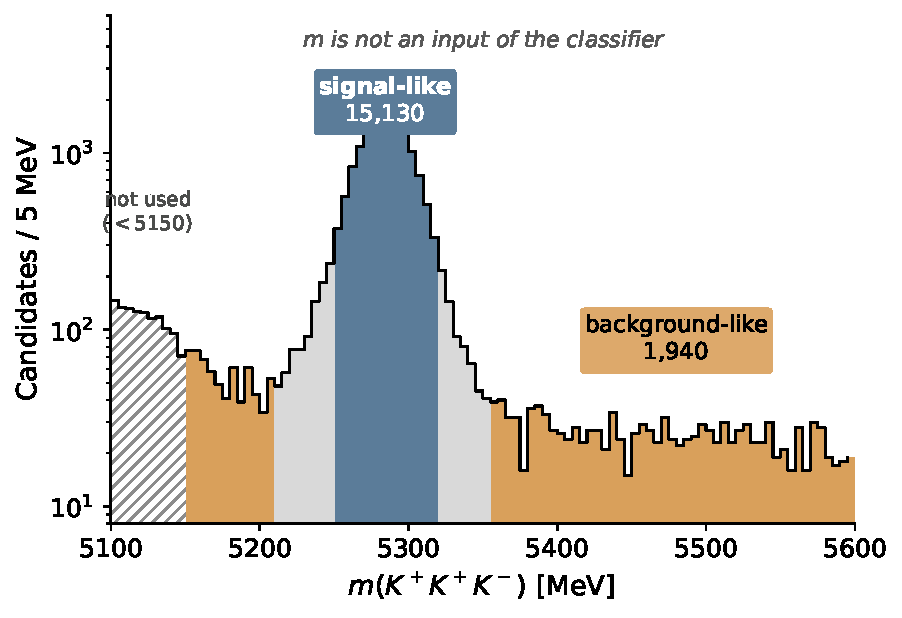
\includegraphics[width=\columnwidth]{figures/short_ml_labels.pdf}
\caption{Weak labels on the mass spectrum of the fit window: signal-like candidates ($|m-\mu|<2\sigma$, $15{,}130$) and background-like candidates (sidebands beyond $4\sigma$ and above $5150\,\MeV$, $1940$); the $2$--$4\sigma$ gap is left unlabeled and the region below $5150\,\MeV$, where the background rises towards partially reconstructed decays, is excluded.}
\label{fig:ml_labels}
\end{figure}

\subsection{Regularization, Bias-Variance and Uncertainty}
\label{sec:ml_regcal_body}
\label{sec:ml_uncertainty_body}
The regularization strength of the logistic regression, scanned over $30$ values of $C=1/\alpha$ with cross-validation, gives the same optimal AUC for the $L1$ and $L2$ penalties ($0.7686$) and no overfitting: the limitation of the linear model is its decision boundary, not the variance. For gradient boosting, whose complexity grows with the number of stages, the test AUC rises up to $\sim150$ stages and then stays at $0.865$ while the training AUC keeps rising (the gap grows from $0.018$ at $20$ stages to $0.084$ at $300$): the additional stages overfit without gain. %Class weights bias the probabilities, which converge to $\tilde p=w_sp/[w_sp+w_b(1-p)]$ instead of $p$; an isotonic recalibration on held-out folds corrects it without changing the ranking.
The uncertainty of a prediction was estimated from the spread of the $300$ trees of the Random Forest, of $300$ forward passes with dropout kept active (MC dropout) and of a deep ensemble of $10$ networks: the mean per-candidate values are $0.178$, $0.095$ and $0.050$; they measure different sources of variability, and only the Random Forest spread decreases visibly with the size of the training set ($0.220$, $0.204$, $0.179$ with a quarter, half and all of it), the epistemic part, while the part at scores around $0.5$ is the aleatoric one.
\subsection{Effect on the Measurement and Dalitz Partition}
\label{sec:ml_stability_body}
\label{sec:ml_kmeans_body}
A cut at $0.5$ on the score keeps $92\%$ of the fitted signal and $36\%$ of the background ($15{,}709$ candidates). The raw asymmetry is \textbf{stable} (Fig.~\ref{fig:ml_three}): $-0.0451\pm0.0087$ (Bayesian) and $-0.0447\pm0.0086$ (Frequentist), against $-0.0443$ and $-0.0441$ for the full window, all shifts within the spread expected for a subsample and $5.2\sigma$ from zero in both samples. The precision does not improve, because the nominal sample has little background to remove ($\approx4\%$ in the signal window). The mass spectrum, instead, changes ($\chi^2$ from $164/88$ to $253/88$ in the Bayesian fit): the classifier does not sculpt the mass, since without the nine momentum components the degradation is the same ($\chi^2=533/388$ in the Frequentist fit), but the selection changes the composition of the background, keeping partially reconstructed decays that the model does not describe. Finally, $K$-means with $K=8$ on $(m^2_{\mathrm{lo}},m^2_{\mathrm{hi}})$, an \emph{unsupervised} partition learned from the density of the candidates and stable between initializations, finds two clusters beyond $3\sigma$ ($\chi^2=46.4$ for $7$ degrees of freedom) with the pattern of the fixed binning ($\chi^2=80.8$ for $31$ degrees of freedom, Sec.~\ref{sec:dalitz}): negative at low $m^2_{\mathrm{lo}}$ ($-0.127\pm0.017$) and positive at high $m^2_{\mathrm{hi}}$ (Fig.~\ref{fig:ml_kmeans}).

\begin{figure}[h]
\centering
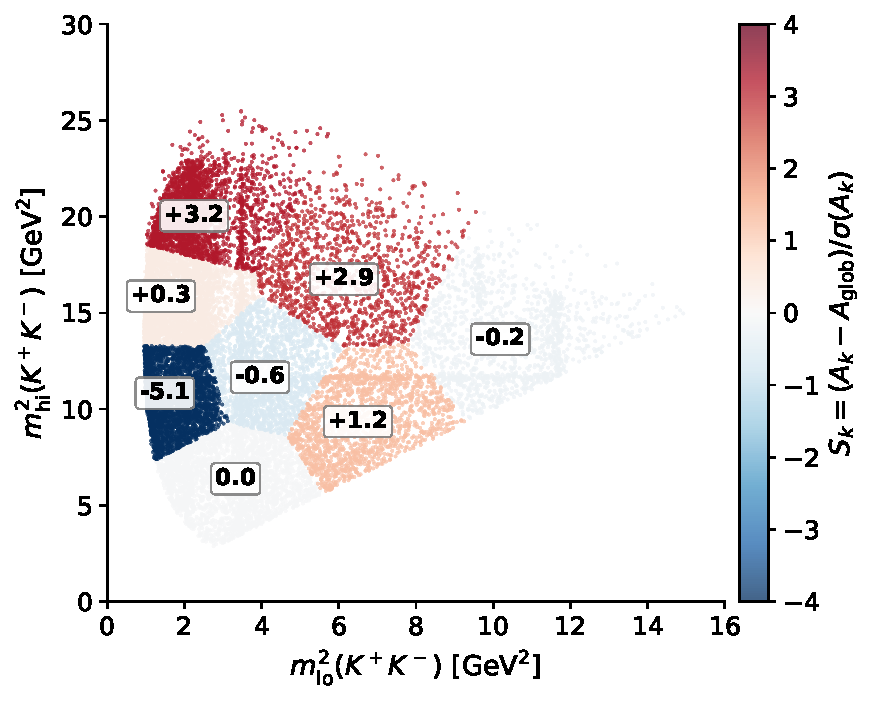
\includegraphics[width=\columnwidth]{figures/short_ml_kmeans.pdf}
\caption{$K$-means partition ($K=8$) of the Dalitz plane, all candidates of the fit window, same axes as Fig.~\ref{fig:bayes_dalitz}. Color and labels: local significance of each cluster with respect to the global asymmetry, $S_k=(A_k-A_{\mathrm{glob}})/\sigma(A_k)$, on the same scale as panel (c) of Fig.~\ref{fig:bayes_dalitz}.}
\label{fig:ml_kmeans}
\end{figure}

\begin{figure}[h]
\centering
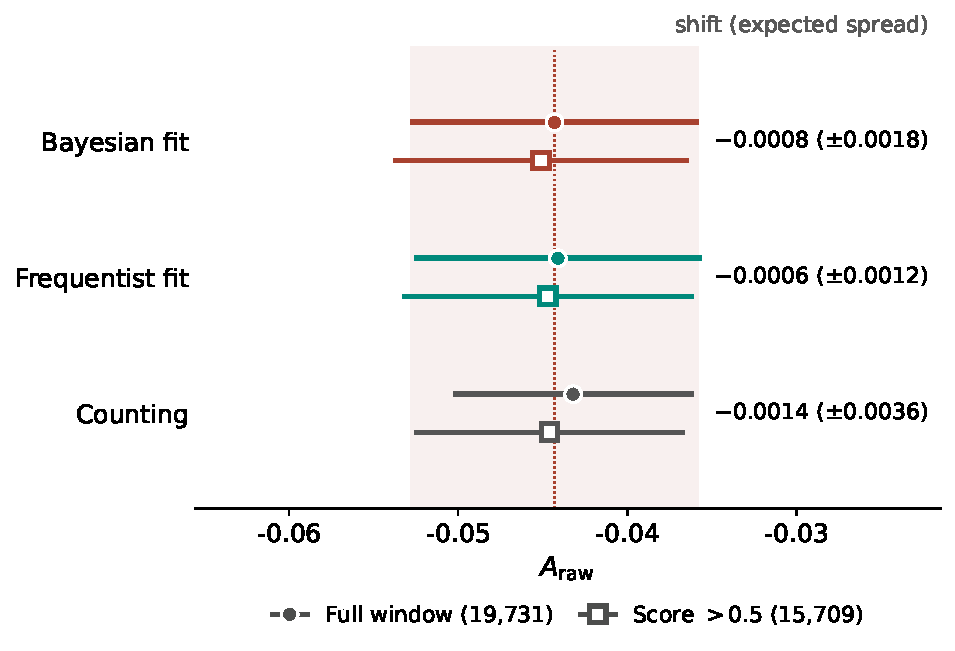
\includegraphics[width=\columnwidth]{figures/short_ml_three.pdf}
\caption{$\Araw$ from the Bayesian fit, the Frequentist fit and counting, for the full sample and the ML-selected ones, at a score cut of $0.5$ and at $0.73$, the maximum of the significance improvement.}
\label{fig:ml_three}
\end{figure}


\section{Local Asymmetry in the Dalitz Plane}
\label{sec:dalitz}
\label{sec:bayes_dalitz}
\emph{In short: the asymmetry is not uniform over the Dalitz plane ($\chi^2=80.8$ for $31$ degrees of freedom) and is concentrated outside the $\phi(1020)$, in the region of the published analysis: $-0.234\pm0.025$ against $-0.239\pm0.020$.}
To test whether the asymmetry is uniform over phase space or concentrated in specific regions, each candidate was placed in the Dalitz plane using the two opposite-sign $K^+K^-$ invariant masses $m^2(H1,H2)$ and $m^2(H1,H3)$ (Sec.~\ref{sec:data_presel}), sorted into $m^2_{\mathrm{lo}}$ and $m^2_{\mathrm{hi}}$ to remove the $H2/H3$ labeling ambiguity. The plane $[0,16]\times[0,30]\,\GeV^2$ in $(m^2_{\mathrm{lo}},m^2_{\mathrm{hi}})$ was divided into an $8\times8$ grid, fixed before looking at the asymmetries. In each bin with at least 20 candidates (32 of 64), the local asymmetry $A_i=(N_i^--N_i^+)/N_i$, with binomial uncertainty $\sigma(A_i)=\sqrt{(1-A_i^2)/N_i}$, was compared with the global counting asymmetry $A_{\mathrm{glob}}=-0.043$ through $S_i=(A_i-A_{\mathrm{glob}})/\sigma(A_i)$.

Figure~\ref{fig:bayes_dalitz} shows the occupancy of the bins (a), the local asymmetry (b) and its significance (c). Two of the 32 bins have $|S_i|>3$, adjacent at $m^2_{\mathrm{lo}}<4\,\GeV^2$ and $7.5<m^2_{\mathrm{hi}}<11.25\,\GeV^2$ ($S_i=-3.7$ and $-3.0$); about $0.09$ such bins would be expected if the asymmetry were uniform, and two or more with probability $3\times10^{-3}$, a look-elsewhere number over any two of the 32 bins. The global homogeneity test, $\chi^2=\sum_iS_i^2=80.8$ for 31 degrees of freedom ($p=3\times10^{-6}$), confirms that the local asymmetry is \textbf{not uniform}; it also holds in the signal window alone, with the charm vetoes and for other grids\appref{app:dalitz_homog}.

\begin{figure*}[t]
\centering
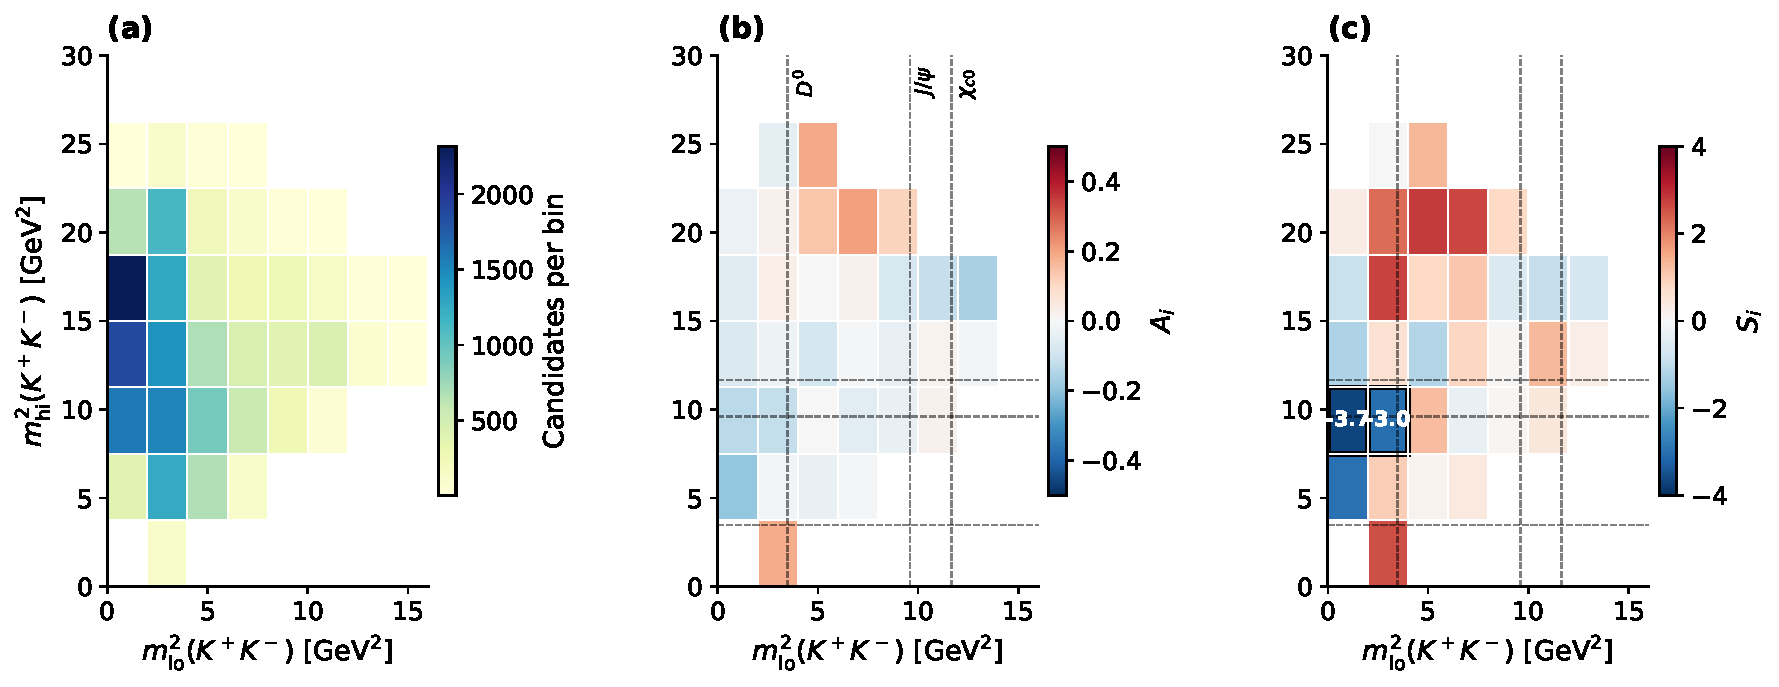
\includegraphics[width=0.95\textwidth]{figures/short_dalitz_maps.pdf}
\caption{Fixed $8\times8$ Dalitz-plot binning, all candidates in the fit window: (a) number of candidates per bin, (b) local asymmetry $A_i$ for bins with $\geq20$ candidates, and (c) local significance with respect to the global asymmetry, $(A_i-A_{\mathrm{glob}})/\sigma(A_i)$. The two bins with $|S_i|>3$ are outlined. Dashed lines: the squared masses of the $D^0$, $J/\psi$ and $\chi_{c0}$, in either opposite-sign pair.}
\label{fig:bayes_dalitz}
\end{figure*}

The structure is the same with both magnet polarities: %in the region of the two significant bins the counting asymmetry is $-0.129\pm0.023$ (magnet down) and $-0.126\pm0.028$ (magnet up), and the two maps agree bin by bin ($\chi^2=23.0$ for 29 bins, $p=0.78$).
the split tests the part of the detection asymmetry that changes sign with the polarity, not the different interaction of $K^+$ and $K^-$ with the detector material.
Where is the asymmetry in terms of the decay dynamics? The Dalitz plane shows the $\phi(1020)$ band at the kinematic edge ($m^2_{\mathrm{lo}}\approx1.04\,\GeV^2$) and the charm bands of the $D^0$, $J/\psi$ and $\chi_{c0}$. The negative asymmetry is \emph{not} produced by the $\phi(1020)$: its band ($1964$ candidates) has $A_{\mathrm{count}}=-0.004\pm0.023$, while the significant bins without it have $-0.145\pm0.019$\appfig{app:dalitz_phi}{Fig.~\ref{fig:dalitz_phi}}. It sits just above the $\phi$, where the published analysis located it, defining the region $1.2<m^2_{\mathrm{lo}}<2.0\,\GeV^2$, $m^2_{\mathrm{hi}}<15\,\GeV^2$ with $\Araw=-0.239\pm0.020$~\cite{lhcb_cpv_2013}. The region is fixed by the paper, not chosen on our data, so the comparison is unbiased: the nominal model fitted to its $2146$ candidates gives $\Araw=\bnum{-0.234\pm0.025}$ (Bayesian) and $-0.237\pm0.025$ (Frequentist, $9.4\sigma$ from zero), reproducing the published value.
%The asymmetries are counts without background subtraction, and part of the local variation can be instrumental\appref{sec:limitations}.

\subsection{Additional Results}
\emph{Null tests.} Permuting the charges gives $\chi^2=31.5\pm8.4$ and never reaches $80.8$ in $2000$ permutations, and the phase-space simulation is consistent with no asymmetry (slightly optimistic $p$-values)\apprefsf{sec:dalitz_null}{app:dalitz_perm}{Fig.~\ref{fig:dalitz_perm}}.

\section{Result and Systematic Uncertainties}
\label{sec:syst}
\emph{In short: thirteen variants in four groups, fitted by both methods on the same candidates, give $0.0070$ (Bayesian) and $0.0072$ (Frequentist), dominated by the particle-identification requirement.}
The result depends on choices of the analysis that the data do not fix. They were varied one at a time in thirteen variants, fitted by both methods on exactly the same candidates and combined with the same rule. The variants fall in four groups: the \emph{window} (lower edge $5050$ and $5150\,\MeV$, upper edge $5450$ and $5700\,\MeV$), the \emph{background} model (single exponential, shape shared between the charges, charge-symmetric background $A_b=0$), the \emph{signal} model (Crystal Ball, $\mu$ and $\sigma$ per charge) and the \emph{preselection} ($\texttt{ProbK}>0.4$ and $0.6$, $\texttt{ProbPi}<0.4$ and $0.6$). When a variant changes the sample (window, preselection) the two samples are nested and part of the shift $\Delta=\Araw^{\mathrm{var}}-\Araw^{\mathrm{nom}}$ is a statistical fluctuation of expected size $\sigma_B=\sqrt{|\sigma_{\mathrm{var}}^2-\sigma_{\mathrm{nom}}^2|}$~\cite{barlow} (the difference of two nearly equal uncertainties, hence sensitive to small differences between the methods: a variant at the threshold can be classified differently without changing the result), so the variant contributes only if $|\Delta|>\sigma_B$; a variant that the data reject (the single exponential) is excluded; the largest remaining $|\Delta|$ of each group is its uncertainty and the groups, being independent choices, are added in quadrature.
The groups give $0.0014$ (window), $0.0037$ (background), $0.0002$ (signal) and $0.0058$ (preselection) in the Bayesian fit and $0.0014$, $0.0040$, $0.0006$ and $0.0058$ in the Frequentist one, for totals of $0.0070$ and $0.0072$; the two methods give the same shifts to within $\sim$$0.0005$. The \textbf{preselection} dominates, through the single variant $\texttt{ProbK}>0.6$ ($+0.0058$, $1.2\,\sigma_B$), which a scan of each cut in steps of $0.05$ shows to be a \emph{fluctuation}: on the tight side the shifts scatter around zero within $1.3\,\sigma_B$ without a trend, whereas loosening $\texttt{ProbK}$ moves $\Araw$ monotonically, as expected if misidentified decays not in the mass model enter the sample (Fig.~\ref{fig:pid_scan_body}). The nominal requirement is therefore well placed and the preselection uncertainty conservative. The shifts of the thirteen variants are shown in Fig.~\ref{fig:syst_variants}, and the final result is
\begin{gather*}
\text{Bayesian:}\\ \Araw=-0.0443\pm0.0085\,(\text{stat})\pm0.0070\,(\text{syst}),\\[2pt]
\text{Frequentist:}\\ \Araw=-0.0441\pm0.0085\,(\text{stat})\pm0.0072\,(\text{syst}).
\end{gather*}

\begin{figure*}[!t]
\centering
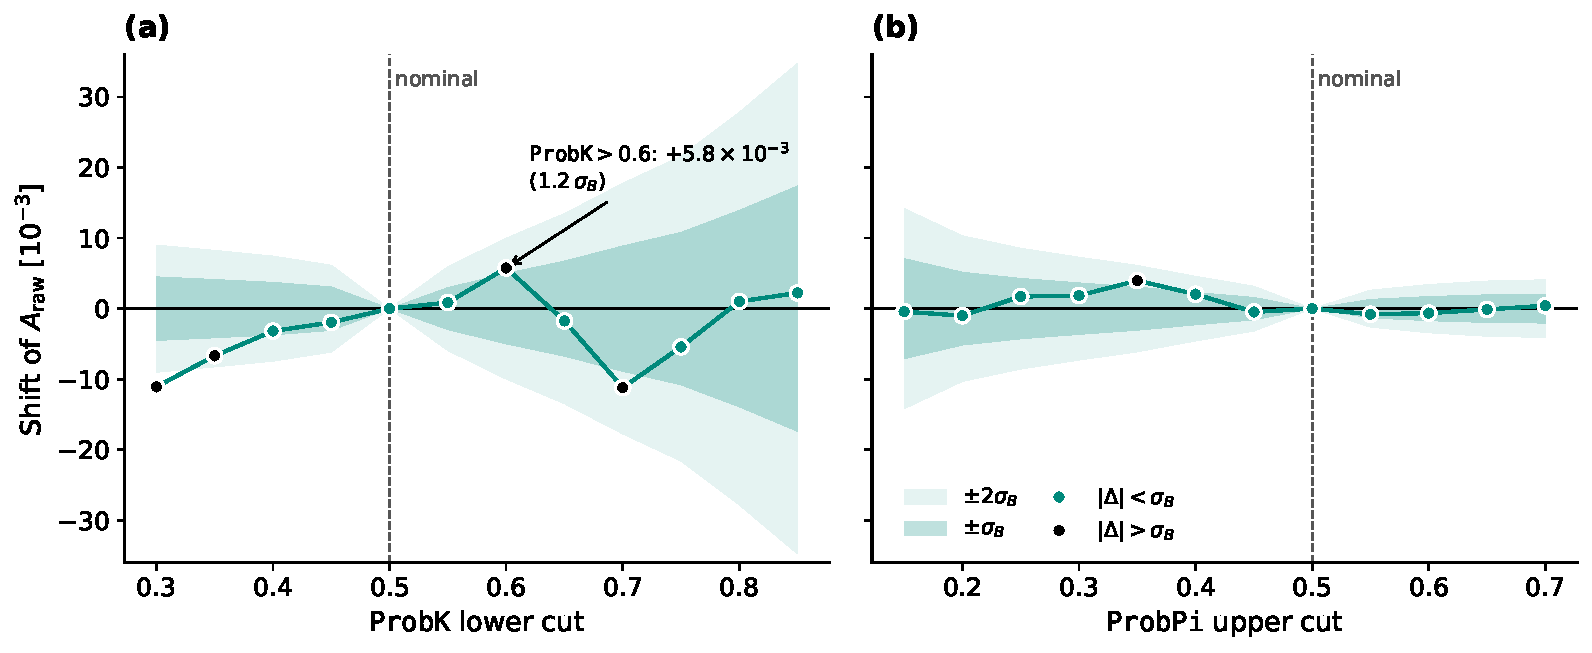
\includegraphics[width=0.80\textwidth]{figures/short_pid_scan.pdf}
\caption{Shift of $\Araw$ (Frequentist fit) as a function of (a) the $\mathtt{ProbK}$ lower cut and (b) the $\mathtt{ProbPi}$ upper cut, in steps of $0.05$, with the expected statistical spread of the nested sample ($\pm\sigma_B$ dark, $\pm2\sigma_B$ light; zero at the nominal cut, dash-dotted line). On the tight side of $\mathtt{ProbK}$ the points scatter around zero without trend and the pion requirement is flat; loosening $\mathtt{ProbK}$ moves $\Araw$ monotonically.}
\label{fig:pid_scan_body}
\end{figure*}

% Fig. XIII (shifts of the variants) and Fig. XIV (profile likelihood and posterior, panels stacked) in one float: one column of figures
\begin{figure}[!t]
\centering
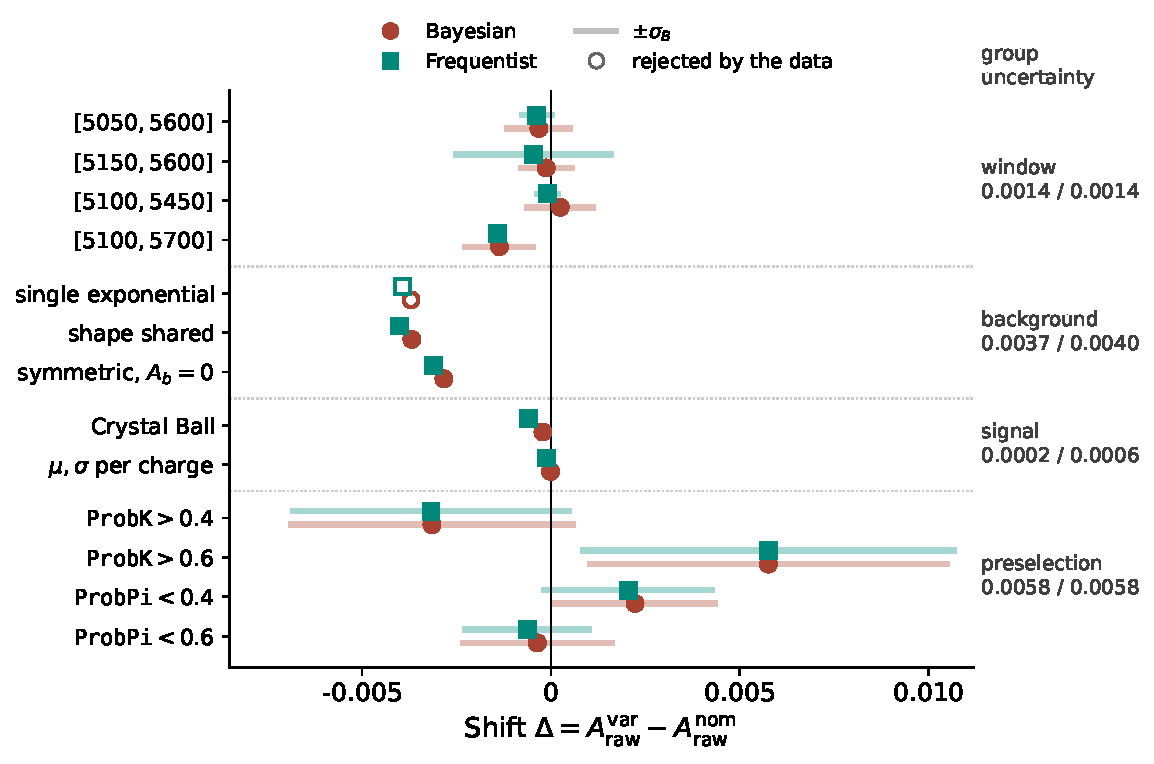
\includegraphics[width=1.0\columnwidth]{figures/short_syst_variants.pdf}
\caption{Shift $\Delta$ of $\Araw$ for the thirteen variants of the analysis, in the Bayesian (circles) and Frequentist (squares) fits, with the expected statistical spread $\sigma_B$ of the variants that change the sample (bars); the open markers are the variant rejected by the data. On the right, the uncertainty of each group (Bayesian / Frequentist), its largest contributing shift.}
\label{fig:syst_variants}

\vspace{6pt}
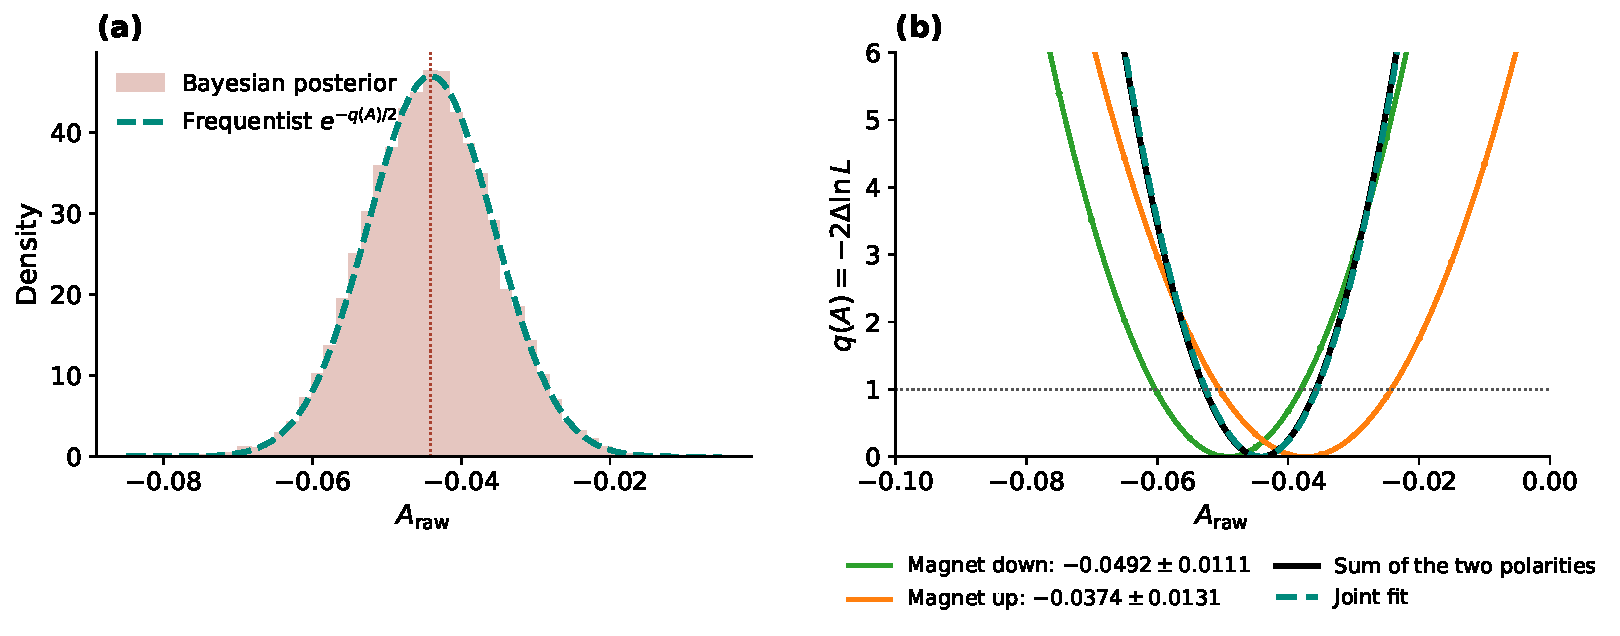
\includegraphics[width=0.8\columnwidth,trim=0 0 398.4bp 0,clip]{figures/short_profile_polarity.pdf}\\[3pt]
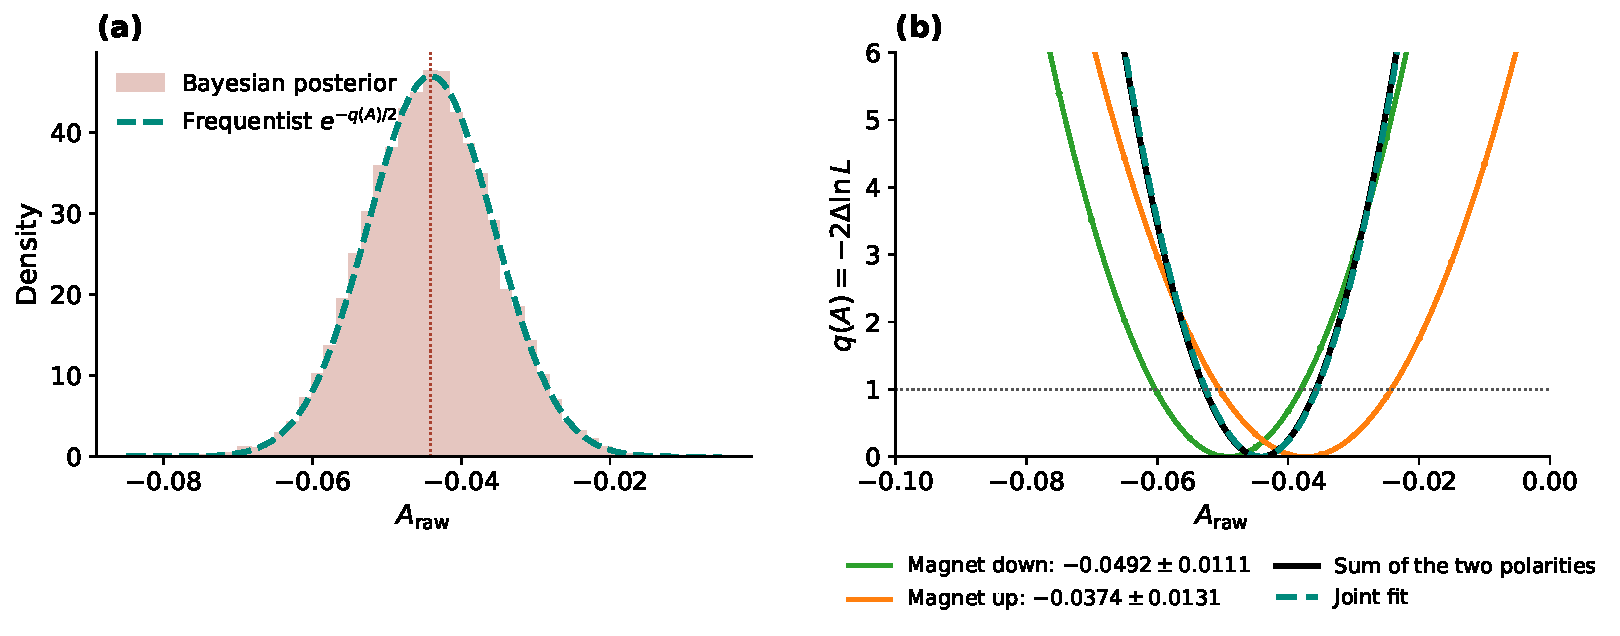
\includegraphics[width=0.8\columnwidth,trim=379bp 0 0 0,clip]{figures/short_profile_polarity.pdf}
\caption{(a) Frequentist profile likelihood, $\exp[-q(A)/2]$ normalized, and Bayesian marginal posterior of $A$: the two coincide. (b) Profile likelihood $q(A)$ of the two magnet polarities (parabolic fits to the points), their sum and the joint fit: the likelihoods of the two polarities combine into that of the full sample.}
\label{fig:checks_profile}
\end{figure}

\subsection{Additional Results}
\emph{Checks.} The $\sigma_B$ rule is verified by bootstrap (the spread of the shift between a sample and its tighter subsample is $\sigma_B$), and the grid scans of the Frequentist fit move $\Araw$ by at most $0.0126$ (PID cuts, smaller samples), $0.0048$ (window edges) and $6\times10^{-5}$ (signal region).

\section{Discussion and Conclusions}
\label{sec:conclusions}
\label{sec:comparison}
\emph{In short: the Frequentist and Bayesian analyses give the same $\Araw=-0.044\pm0.009\,(\text{stat})\pm0.007\,(\text{syst})$, $5.2$ standard deviations from zero, with validated intervals; they differ in the meaning of the numbers and of the tests, not in their values.}
On this problem the Frequentist profile-likelihood fit and the Bayesian posterior are equivalent in value, uncertainty and coverage: with a common selection and mass model they give $\Araw=-0.0441\pm0.0085\pm0.0072$ and $-0.0443\pm0.0085\pm0.0070$ (statistical, systematic), a nonzero asymmetry at $5.2$ standard deviations, stable under the thirteen variants (the dominant systematic contribution is the particle-identification requirement) and concentrated in the Dalitz region of the published analysis outside the $\phi(1020)$ ($-0.234\pm0.025$ against $-0.239\pm0.020$).
\textbf{The numbers coincide, the statements do not.} The \emph{credible interval} states that $A$ lies in $[-0.0528,-0.0358]$ with $68\%$ probability given the data and the prior; the \emph{confidence interval} $[-0.0526,-0.0356]$ is the set of values that the data do not reject, and its $68\%$ is verified by the bootstrap and the toy experiments. The Frequentist test of $A=0$, $p=2\times10^{-7}$, is independent of the prior; the Bayes factor, $BF_{10}\approx9\times10^3$, depends on its width (Sec.~\ref{sec:bayes_factor}), and for $A_b=-0.040\pm0.018$ a Frequentist test would call $2.3\sigma$ a hint while $BF_{01}\approx3.5$ mildly favors $A_b=0$. The Frequentist fit adds an unbiased estimator at the minimum variance bound; the Bayesian analysis adds sampling diagnostics and a posterior predictive check. Figure~\ref{fig:checks_profile} shows the profile likelihood and the marginal posterior of $A$ on the same axis, and the likelihoods of the two magnet polarities.

\label{sec:comparison_published}
The published analysis~\cite{lhcb_cpv_2013} finds $-0.060\pm0.007$ on a larger sample ($22{,}119\pm164$ signal candidates) with a richer model (a Cruijff signal and misidentified and partially reconstructed backgrounds); with the same $D^0$ veto the Bayesian fit gives $-0.0496\pm0.0088$, within $0.93\sigma$. The raw asymmetry is not the $CP$ asymmetry, $\ACP\approx\Araw-A_P-A_D$ (Eq.~\eqref{eq:acp}; in the published analysis the corrections move $-0.060$ to $-0.043\pm0.009 \,\text{(stat)}\pm0.003\,\text{(syst)}\pm0.007\,\text{($J/\psi\, K^{\pm}$)}$ and cannot be assumed for a different selection): the $5.2\sigma$ here is the significance of a nonzero raw asymmetry, not of $CP$ violation. Four limitations bound the result: no tested model reaches $\chi^2/\mathrm{ndof}\approx1$, although $\Araw$ does not depend on the signal shape; no production or detection correction is applied (the record has no control channel, and its other three channels are not analysed); the local Dalitz-plane asymmetries are counts without background subtraction; and the machine-learning labels are weak and imbalanced. A machine-learning selection leaves $\Araw$ unchanged within its statistical spread (Sec.~\ref{sec:ml_body}), and the natural next step is a control-channel correction.
\subsection{Additional Results}
\emph{Numerical agreement.} The estimates of the two fits differ by $0.0002$, both uncertainties are $0.0085$, and sideband subtraction gives $-0.0503\pm0.0083$.
\emph{Profile, posterior and polarities.} Profiling and marginalizing the eleven nuisance parameters give the same distribution of $A$, since $A$ is almost uncorrelated with them; the two polarities agree and their combined likelihood reproduces the joint fit; the $68\%$ and $95\%$ regions in $(A,A_b)$ of the profile ($\Delta\mathrm{NLL}$ at $2.30$ and $5.99$) and of the highest posterior density coincide, with $A=0$ outside both.
\emph{Tests and goodness of fit.} The exact binomial test of $N^-=N^+$ on all $19{,}731$ candidates ($A_{\mathrm{count}}=-0.0432\pm0.0071$) gives $6.1\sigma$, larger than the $5.2\sigma$ of the fit ($-0.0441\pm0.0085$), and the two are not in tension: the count tests the charge asymmetry of signal and background together, without the mass, so its uncertainty does not include the cost of separating the background, while the fit tests the asymmetry of the signal alone with that of the background free; the $5.2\sigma$ is the one that refers to the signal. The same fit has $p=0.03$ in $2.5\,\MeV$ bins and $p\approx5\times10^{-6}$ in $10\,\MeV$ bins: the $p$-value of the binned $\chi^2$ depends on the binning as much as on the model.
\emph{Low statistics.} Credible and confidence intervals coincide in value and coverage from $\sim2\times10^4$ down to $50$ candidates.
%\emph{Published analysis.} It has $22{,}119\pm164$ signal candidates, a Cruijff signal and misidentified and partially reconstructed backgrounds; its corrections move $-0.060$ to $-0.043\pm0.009\pm0.003\pm0.007$ and cannot be assumed for another selection.


\bibliography{biblio}

\end{document}
